%%%%%%%%%%%%
%
% $Autor: Zarzycki $
% $Datum: 2025-09-26 11:30:00Z $
% $Pfad: TemplateSensor $
% $Version: 4250 $
% !TeX spellcheck = en_GB/de_DE
% !TeX encoding = utf8
% !TeX root = filename 
% !TeX TXS-program:bibliography = txs:///biber
%
%%%%%%%%%%%%

% Structure
\chapter{Temperatursensor DS18B20}
	Dieses Kapitel beschreibt den digitalen Temperatursensor DS18B20, seine Eigenschaften und seine Einbindung in ein 1-Wire-System. Es werden Aufbau, Funktionsweise, Speicherstruktur, Auflösungsmodi, Alarmfunktionen und der 64-Bit-ROM-Code erläutert. Darüber hinaus werden Stromversorgungsarten, Verdrahtung mit dem Arduino MKR WAN 1310 sowie der Funktionsbefehlssatz dargestellt. Abschlie{\ss}end folgen Bibliotheksunterstützung, Beispielprogramme für Temperaturmessung und Alarmüberwachung sowie eine objektorientierte Umsetzung für mehrere Sensoren.
	
\section{Allgemeines}
Temperatursensoren sind weit verbreitete Geräte, deren Nachfrage in verschiedensten Bereichen kontinuierlich steigt \cite{MAM:2025}. Sie sind Bestandteil vieler Alltagsgeräte wie \textit{Heating, Ventilation and Air Conditioning (HVAC)} -Systeme \cite{Shinoda:2021}, Automobile \cite{Zun:2011} und Wasserkocher. Darüber hinaus finden sie in industriellen sowie wissenschaftlichen Systemen Verwendung, etwa in Energieanlagen wie Atomkraftwerken \cite{Hashemian:2009}, bei der Überwachung elektrischer Leitungen \cite{Navarrete:2025}, in der Luftfahrt \cite{Zhang:2024} oder in der Lebensmittelindustrie \cite{Wan:2024}, wo häufig nicht nur ein, sondern mehrere Sensoren gleichzeitig eingesetzt werden \cite{Lin:2002}.

Temperatursensoren wandeln thermische Energie in elektrische Signale (z. B. Spannung, Widerstand oder Strom (\cite[3]{Fraden:2010})) um, die gemessen und ausgewertet werden können \cite[519 -- 520]{Fraden:2010}. Dabei existiert eine Vielzahl von Modellen (NTC- und PTC-Thermistoren, digitale Thermometer, Thermoelemente), die für unterschiedliche Einsatzumgebungen ausgelegt sind und verschiedene Kommunikationsprotokolle unterstützen. \cite[1]{Elyounsi:2021}.
	


\section{Temperatursensor DS18B20}
Der Temperatursensor DS18B20 zeichnet sich durch eine direkte Umwandlung der gemessenen Temperaturen in digitale Signale aus. Dadurch ist keine Kalibrierung erforderlich, und der Sensor liefert die Temperatur unmittelbar in Grad Celsius. Er bietet eine wählbare Auflösung zwischen 9 und 12 Bit und ermöglicht die Definition von oberen und unteren Temperaturgrenzen für Alarmmeldungen über nichtflüchtige, benutzerprogrammierbare Triggerpunkte. Die Kommunikation erfolgt über den \textit{1-Wire}-Bus, wodurch sich mehrere Sensoren parallel an einer einzigen Datenleitung betreiben lassen. Die Verwendung des \textit{1-Wire}-Protokolls erlaubt zudem den Einsatz über grö{\ss}ere Distanzen (laut \cite{Navarrete:2025} bis zu etwa 100 m), da Spannungsabfälle und Störeinflüsse, wie sie bei analogen Sensoren auftreten können \cite{Richelli:2015}, vermieden werden \cite{Maxim:2019}.

Zusätzlich kann der DS18B20 im sogenannten \textit{Parasite Mode} arbeiten, bei dem die Energieversorgung direkt über die Datenleitung erfolgt. Jeder Sensor verfügt über eine eindeutige 64-Bit-Seriennummer, die eine klare Identifikation einzelner Sensoren am selben Bus ermöglicht. Dies gestattet es einem Mikrocontroller, eine Vielzahl von Sensoren effizient und zuverlässig zu verwalten \cite{Fezari:2019} \cite[3]{Elyounsi:2021}. 

	\begin{figure}[H]
		\centering
		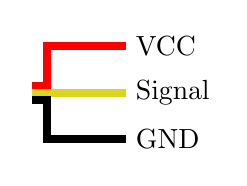
\begin{tikzpicture}
			\temperatureSensorGeneral{1.4}{0}{0}{0}
			\draw[line width=0.1cm, red] (8.4, 0.09) -- ++(0.2, 0) -- ++(0, 0.5) -- ++(1, 0) coordinate (ds18b20-VCC);
			\draw[line width=0.1cm, yellow!85!black] (8.4, 0.0) -- ++(1.2, 0) coordinate (ds18b20-Signal);
			\draw[line width=0.1cm, black] (8.4, -0.09) -- ++(0.2, 0) -- ++(0, -0.5) -- ++(1, 0) coordinate (ds18b20-GND);
			
			\node[right] at (ds18b20-VCC) {VCC};
			\node[right] at (ds18b20-Signal) {Signal};
			\node[right] at (ds18b20-GND) {GND};
		\end{tikzpicture}
		\caption{Temperatursensor DS18B20}
		\label{fig:ds18b20-pinout}
	\end{figure}
	
	
Die Abbildung \ref{ds18b20:blockdiagramm} zeigt das Blockdiagramm des DS18B20-Sensors. Der integrierte 64-Bit-ROM speichert die eindeutige Seriennummer des Sensors. Im Scratchpad-Speicher (Zwischenspeicher) befindet sich ein 2-Byte-Temperaturregister, in dem der digitale Ausgangswert des Temperatursensors abgelegt wird. Darüber hinaus umfasst das Scratchpad weitere Speicherbereiche: je ein 1-Byte-Register für die obere und untere Alarmschwelle ($T_H$ und $T_L$) sowie ein 1-Byte-Konfigurationsregister. Letzteres ermöglicht die Einstellung der Temperatur-Digital-Umwandlung mit einer Auflösung von 9, 10, 11 oder 12 Bit. Die Konfigurationsregister, $T_H$- und $T_L$-Register sind als nichtflüchtige Speicher (EEPROM) ausgeführt und behalten ihre Werte auch nach dem Abschalten der Versorgungsspannung bei \cite{Maxim:2019}.

\begin{figure}[H]
	\centering
	\resizebox{\textwidth}{!}{%
		\begin{tikzpicture}
			\dsTempSensorBlockDiagramm
		\end{tikzpicture}%
	}
	\caption{Blockdiagramm des DS18B20-Sensors  \cite{Maxim:2019}}
	\label{ds18b20:blockdiagramm}
\end{figure}


\begin{figure}[H]
	\centering
	\resizebox{0.85\textwidth}{!}{%
			\fbox{
			\begin{tikzpicture}
				\dsMemoryMap
			\end{tikzpicture}%
		}
	}
	\caption{Blockdiagramm des DS18B20-Zwischenspeichers  \cite{Maxim:2019}}
	\label{ds18b20:memoryMapp}
\end{figure}


\subsection{Stromversorgung}
	Der DS18B20 kann in zwei Konfigurationen betrieben werden:
	\begin{enumerate}
		\item im \textit{Parasite Mode}
		\item mit externer Stromversorgung
	\end{enumerate}
	
	Unabhängig von der Betriebsart muss die Signalleitung des 1-Wire-Busses mithilfe eines schwachen Pull-up-Widerstands (typischerweise 4,7~k$\Omega$) auf logisches \textit{High} gezogen werden. Dieser stellt sicher, dass die Leitung in Ruhephasen einen definierten High-Pegel annimmt, da die 1-Wire-Ausgänge als Open-Drain ausgeführt sind und selbst keinen High-Pegel treiben können.


\subsubsection{Parasite Mode \label{lab:parasiteMode}}
	Im Parasite Mode ist der Pin $V_{DD}$ des DS18B20 direkt mit GND verbunden, sodass der Sensor seine gesamte Energie über die Datenleitung bezieht. Während die Leitung auf High-Pegel liegt, lädt das interne \textit{Parasite Power Circuit} einen Kondensator auf, der den Sensor in Phasen mit Low-Pegel weiter versorgt.
	
	Diese Konfiguration ermöglicht einen minimalen Verdrahtungsaufwand und eignet sich daher besonders für platzkritische Anwendungen oder Umgebungen mit sehr wenigen Leitungen.
	
	Allerdings ist die Leistungsaufnahme des Sensors während bestimmter Operationen deutlich erhöht, insbesondere bei Temperaturkonvertierungen oder beim Schreiben ins \ac{eeprom}. In diesen Fällen reicht der Strom über den Pull-up-Widerstand nicht aus. Daher muss der Bus spätestens $10\,\mu\text{s}$ nach einem \texttt{Convert T [44h]}- oder \texttt{Copy Scratchpad [48h]}-Befehl (siehe \autoref{dsCommandSet}) auf einen sogenannten \textit{strong pull-up} umgeschaltet werden. Dies geschieht typischerweise mithilfe eines MOSFETs, der die Leitung aktiv auf die Versorgungsspannung zieht. Der erhöhte Pull-up-Pegel muss für die gesamte Dauer der jeweiligen Operation aufrechterhalten werden, während keine weitere Kommunikation auf dem Bus stattfinden darf.

\subsubsection{Externe Stromversorgung \label{lab:extPowered}}
	Wird der DS18B20 über den Pin $V_{DD}$ direkt mit einer Versorgungsspannung betrieben, übernimmt dieser die Stromversorgung des Sensors. In dieser Betriebsart dient der Pull-up-Widerstand ausschlie{\ss}lich zur Pegelsteuerung der Datenleitung, da kein Energiebedarf über die Busleitung gedeckt werden muss.
	
	Der gro{\ss}e Vorteil dieser Konfiguration besteht darin, dass während Temperaturkonvertierungen oder Schreibvorgängen ins \ac{eeprom} keine zusätzlichen Ma{\ss}nahmen wie ein starker Pull-up erforderlich sind. Der 1-Wire-Bus bleibt vollständig für weitere Kommunikation nutzbar, was insbesondere in Systemen mit mehreren Sensoren oder kontinuierlichem Datenaustausch entscheidend ist. \cite{Maxim:2019}, \cite{Texas:2025}.
	
	In diesem Kapitel wird ausschlie{\ss}lich die Methode der externen Stromversorgung verwendet und durch weitere Beispiele verdeutlicht.

\subsection{Funktionsweise}
	Der grö{\ss}te Vorteil dieses Sensors liegt in seiner direkten Temperatur-zu-Digital-Konvertierung. Die wählbare Auflösung von 9, 10, 11 oder 12 Bit entspricht einer Genauigkeit von $0{,}5 ^\circ\mathrm{C}$, $0{,}25 ^\circ\mathrm{C}$, $0{,}125 ^\circ\mathrm{C}$ beziehungsweise $0{,}0625 ^\circ\mathrm{C}$. Standardmä{\ss}ig beträgt die Auflösung nach dem Einschalten 12 Bit. Der Sensor startet im Low-Power-Idle-State, was bedeutet, dass er unmittelbar nach dem Einschalten keine Messungen durchführt, sondern auf Befehle des Masters wartet. Sobald der Befehl von Master zur Temperaturmessung erteilt wird, führt der DS18B20 die Messung durch, speichert das Ergebnis im 2-Byte-Temperaturregister und wechselt anschlie{\ss}end wieder in den Idle-Modus.
	Wird der Sensor mit einer \hyperref[lab:extPowered]{externen Spannungsversorgung} betrieben, kann der Master während der Konversion abfragen, ob diese bereits abgeschlossen ist, und anschlie{\ss}end den Temperaturwert auslesen. Im \hyperref[lab:parasiteMode]{Parasite Mode} hingegen muss die vollständige Konversionszeit abgewartet werden (vgl. \autoref{ds18b20:conversionTimes}), bevor der Master den Messwert beim Sensor abruft.
	
	Der Sensor gibt die Temperatur in Grad Celsius zurück. Der Wert wird als 16-Bit-Zahl im Zweierkomplement mit Vorzeichenerweiterung (sign-extended two's complement) im Temperature Register abgelegt (siehe \autoref{fig:dsTempRegister}). Die höchstwertigen fünf Bits dienen als Vorzeichenbits (S) und zeigen an, ob die Temperatur positiv (S = 0) oder negativ (S = 1) ist.
	Die verbleibenden Bits (10 - 0) enthalten den Messwert, wobei die tatsächlich genutzte Bitanzahl von der eingestellten Auflösung abhängt:
	\begin{itemize}
		\item 12-Bit-Auflösung $\rightarrow$ alle Bits (10 - 0) sind definiert
		\item 11-Bit-Auflösung $\rightarrow$ Bit 0 undefiniert
		\item 10-Bit-Auflösung $\rightarrow$ Bit 1 und Bit 0 undefiniert
		\item 9-Bit-Auflösung $\rightarrow$ Bit 2, Bit 1 und Bit 0 undefiniert
	\end{itemize}
	
	\begin{figure}[H]
		\centering
		\resizebox{\textwidth}{!}{%
			\fbox{
				\begin{tikzpicture}
					\dsTempRegisterFormat
				\end{tikzpicture}%
			}
		}
		\caption{Bitstruktur des Temperatur-Registers (MS-Byte und LS-Byte) des DS18B20}
		\label{fig:dsTempRegister}
	\end{figure}

	Die \autoref{tab:dsTemperaturOutputBytesExample} zeigt die Bitanordnung im 16-Bit-Ausgabeformat des DS18B20 für ausgewählte Temperaturmessungen.
	
	\begin{table}[H]
		\centering
		\begin{tabular}{|c|c|}
			\hline
			\textbf{Temperatur} & \textbf{Digitaler Ausgang (Binär, 16 Bit)} \\
			\hline
			$+85^\circ\mathrm{C}$ & 0000 0101 0101 0000 \\
			\hline
			$+25.0625^\circ\mathrm{C}$ & 0000 0001 1001 0001 \\
			\hline
			$+10.125^\circ\mathrm{C}$  & 0000 0000 1010 0010 \\
			\hline
			$+0.5^\circ\mathrm{C}$ & 0000 0000 0000 1000 \\
			\hline
			$0^\circ\mathrm{C}$ & 0000 0000 0000 0000 \\
			\hline
			$-0.5^\circ\mathrm{C}$ & 1111 1111 1111 1000 \\
			\hline
			$-10.125^\circ\mathrm{C}$  & 1111 1111 0101 1110 \\
			\hline
			$-25.0625^\circ\mathrm{C}$ & 1111 1110 0110 1111 \\
			\hline
			$-55^\circ\mathrm{C}$      & 1111 1100 1001 0000 \\
			\hline
		\end{tabular}
		\caption{Beispiele für Temperaturwerte im Digitalformat des DS18B20 (16-Bit, Two's Complement) \cite{Maxim:2019}}
		\label{tab:dsTemperaturOutputBytesExample}
	\end{table}


\subsection{Alarmbenachrichtigung \label{alarmTriggerFeature}}
Nach jeder Temperaturmessung wird der im \textit{Temperatur-Register} gespeicherte Wert mit den vom Benutzer definierten unteren ($T_L$) und oberen ($T_H$) Alarmschwellen verglichen. 
Standardmä{\ss}ig ist $T_L$ auf \(-55\,^\circ\mathrm{C}\) und $T_H$ auf \(+125\,^\circ\mathrm{C}\) gesetzt. 

Die $T_H$- und $T_L$-Register sind als nichtflüchtige Speicher (EEPROM) ausgeführt und behalten ihre Werte auch nach dem Abschalten der Versorgungsspannung bei.

Da es sich bei den $T_H$- und $T_L$-Registern um 8-Bit-Register handelt (siehe \autoref{fig:dsAlarmRegisterFormat}), können sie nur ganze Zahlen repräsentieren. Das Vorzeichenbit gibt an, ob die gespeicherte Temperatur positiv oder negativ ist: $S = 1$ für negative und $S = 0$ für positive Werte. 
Daher erfolgt der Vergleich ausschlie{\ss}lich mit den Bits 10 - 4 des \textit{Temperatur-Registers} (siehe \autoref{fig:dsTempRegister}), was die Auflösung auf Ganzzahlen reduziert.

Liegt die gemessene Temperatur oberhalb oder gleich $T_H$ bzw. unterhalb oder gleich $T_L$, wird ein internes Alarm-Flag auf \textit{true} gesetzt. 
Dieses Flag wird nach jeder neuen Messung aktualisiert, kehrt der Wert in den sicheren Bereich zurück, wird das Flag automatisch zurückgesetzt. 

Die Alarmbenachrichtigung kann den Datenverkehr auf dem 1-Wire-Bus erheblich reduzieren, da der Master nicht mehr jeden Sensor einzeln abfragen muss. 
Es genügt, wenn der Master den Befehl \textit{Alarm Search [ECh]} (siehe \autoref{dsCommandSet}) ausführt. 
Daraufhin antworten ausschlie{\ss}lich die Sensoren, bei denen das Alarm-Flag gesetzt ist. 
Auf diese Weise können gezielt nur die betroffenen Sensoren überprüft und weiter überwacht werden.

\begin{figure}[H]
	\centering
	\resizebox{\textwidth}{!}{%
		\fbox{
			\begin{tikzpicture}
				\dsAlarmRegisterFormat
			\end{tikzpicture}%
		}
	}
	\caption{Bitstruktur des $T_L$ und $T_H$ Registers des DS18B20}
	\label{fig:dsAlarmRegisterFormat}
\end{figure}

\subsection{Konfigurationsregister}
	Byte 4 des Scratchpads (siehe \autoref{ds18b20:memoryMapp}) ist das Konfigurationsregister, in dem die Auflösung eingestellt wird. Die Bits 7 sowie 4 bis 0 sind reserviert (siehe \autoref{fig:dsConfigRegisterFormat}) und dürfen nicht überschrieben werden.
	
	\begin{figure}[H]
		\centering
		\resizebox{\textwidth}{!}{%
			\fbox{
				\begin{tikzpicture}
					\dsConfigRegisterFormat
				\end{tikzpicture}%
			}
		}
		\caption{Bitstruktur des Konfigurationsregisters des DS18B20}
		\label{fig:dsConfigRegisterFormat}
	\end{figure}
	
	Die \autoref{tab:BytesResoltionConfig} zeigt, welche Bitkombinationen im Konfigurationsregister die jeweilige Auflösung bestimmen.

	\begin{table}[H]
		\centering
		\begin{tabular}{|c|c|c|}
			\hline
			\textbf{R1} & \textbf{R0} & \textbf{Auflösung} \\
			\hline
			0 & 0 & 9 Bit\\
			\hline
			0 & 1 & 10 Bit\\
			\hline
			1 & 0 & 11 Bit\\
			\hline
			1 & 1 & 12 Bit\\
			\hline
		\end{tabular}
		\caption{Darstellung der Bits im Konfigurationsregister abhängig von der gewählten Auflösung}
		\label{tab:BytesResoltionConfig}
	\end{table}
	
	
\subsection{64-Bit gelaserter ROM-Code}
Jeder DS18B20 verfügt über einen eindeutigen, im ROM gespeicherten 64-Bit-Code (siehe Abbildung~\ref{ds18b20:blockdiagramm}). Wie in \autoref{fig:dsLaseredRomCode} dargestellt, enthalten die niederwertigsten 8 Bits den \textit{1-Wire Family Code} des DS18B20. Darauf folgen 48 Bits, die die individuelle Seriennummer des Sensors repräsentieren. Die höchstwertigen 8 Bits bilden einen Cyclic Redundancy Check (CRC), der aus den ersten 56 Bits berechnet wird und zur Integritätsprüfung des Codes dient.

	\begin{figure}[H]
		\centering
		\resizebox{\textwidth}{!}{%
			\begin{tikzpicture}
				\dsLaseredRomCode
			\end{tikzpicture}%
		}
		\caption{Struktur des gelaserter ROM-Codes}
		\label{fig:dsLaseredRomCode}
	\end{figure}

\subsubsection{1-Wire Family Code}
	Der \textit{Family Code} informiert den Master darüber, um welchen Sensortyp es sich handelt. 
	Da am 1-Wire-Bus viele verschiedene Sensoren und Geräte betrieben werden können, muss sich jedes Gerät eindeutig identifizieren lassen. 
	Für den DS18B20 ist der 1-Wire Family Code auf \texttt{28h} (binär: 00101000) festgelegt. 
	Anhand dieses Codes erkennt der Master, dass es sich bei dem Gerät um einen Temperatursensor vom Typ DS18B20 handelt.


\subsubsection{Individuelle Seriennummer des Sensors}
	Jeder DS18B20 verfügt über eine weltweit eindeutige 48-Bit-Seriennummer,  die vom Hersteller während der Produktion fest in den Chip eingebrannt (laserprogrammiert) wird und nicht verändert werden kann. Befinden sich mehrere Sensoren am selben 1-Wire-Bus, kann der Master sie anhand ihrer Seriennummer eindeutig unterscheiden. So ist sichergestellt, dass jeder Sensor gezielt adressiert und abgefragt werden kann. 
		

\subsubsection{Cyclic Redundancy Check (CRC)}
	Der CRC dient der Überprüfung der Übertragungskorrektheit. Aus den übertragenen Daten wird eine Prüfsumme berechnet, die zusammen mit den Daten gespeichert oder gesendet wird. Der Master kann diese Prüfsumme ebenfalls berechnen und mit dem empfangenen Wert vergleichen. Stimmen beide überein, ist sichergestellt, dass die Daten fehlerfrei übertragen wurden.  

	Beim DS18B20 kommt der CRC in zwei Fällen zum Einsatz:  
	\begin{itemize}
		\item \textbf{ROM-CRC:} Die oberen 8 Bit des 64-Bit-ROM-Codes (siehe \autoref{fig:dsLaseredRomCode}) enthalten einen CRC, der über die ersten 56 Bit (Family Code und Seriennummer) berechnet wird (dieser CRC wird bei der Sensoradressierung verwendet).
		\item \textbf{Scratchpad-CRC:} Das neunte Byte des Scratchpads (siehe \autoref{ds18b20:memoryMapp})speichert einen CRC, der aus den ersten acht Bytes des Scratchpads (Temperaturregister, Alarmgrenzen, Konfigurationsregister) berechnet wird (dieser CRC wird bei der Datenübertragung verwendet).
	\end{itemize}



\section{Specification}
\subsection{Technische Daten}
\begin{table}[H]
	\centering
	\begin{tabular}{|c|c|}
		\hline
		Gehäusematerial & Edelstahl \\
		\hline
		Eingebauter Temperatursensor & DS18B20 \\
		\hline
		Versorgungsspannung & 3 V - 5.5V \\
		\hline
		Betriebstemperatur & von $-55\,^\circ\mathrm{C}$ bis $+125\,^\circ\mathrm{C}$ \\
		\hline
		Genauigkeit & \pm $0,5\,^\circ\mathrm{C}$ im Bereich von $-10\,^\circ\mathrm{C}$ bis $85\,^\circ\mathrm{C}$ \\
		\hline
		Schnittstelle & 1-Wire\\
		\hline
		Sondenabmessungen & 6 x 50{,}mm\\
		\hline
	\end{tabular}
	\caption{Temperatursensor DS18B20 - Parameter}	% <- BIB
\end{table}		

\subsection{Genauigkeit und Konversionzeit}
\begin{table}[H]
	\centering
	\begin{tabular}{|c|c|c|}
		\hline
		\textbf{Auflösung} & \textbf{Maximale Konversionzeit (ms)} & \textbf{Genauigkeit}\\
		\hline
		9 - Bit Auflösung & 93.75 & $0{,}5,^\circ\mathrm{C}$\\
		\hline
		10 - Bit Auflösung& 187.5 & $0{,}25,^\circ\mathrm{C}$\\
		\hline
		11 - Bit Auflösung& 375 & $0{,}125,^\circ\mathrm{C}$ \\
		\hline
		12 - Bit Auflösung& 750 & $0{,}0625,^\circ\mathrm{C}$\\
		\hline
	\end{tabular}
	\caption{Konversionzeit}
	\label{ds18b20:conversionTimes}
\end{table}

\subsection{Pinbelegung}
\begin{table}[H]
	\centering
	\begin{tabularx}{\textwidth}{|X|c|c|}
		\hline
		\textbf{Beschreibung} & \textbf{Kabelfarbe} & \textbf{Bezeichnung} \\
		\hline
		Optionale Stromversorgung des Sensors (3 V bis 5,5 V). Muss für den Betrieb im \textit{Parasite Mode} auf Masse gelegt werden & rot & $V_{DD}$\\
		\hline
		Masse (GND) des Systems & schwarz & GND\\
		\hline
		Signalkabel (Datenleitung). Versorgt das Gerät mit Energie, wenn es im \textit{Parasite Mode} betrieben wird & gelb & $D_Q$ \\
		\hline
	\end{tabularx}
	\caption{Kabelfarben des DS18B20-Sensors}
\end{table}

\section{Anschluss an Arduino MKR WAN1310}	
	Um die Komplexität zu reduzieren und eine effiziente Lösung zu nutzen, wird hier die Schaltung für die Variante mit externer Spannungsversorgung dargestellt (siehe \autoref{lab:extPowered}). Die Signalleitung kann an einem beliebigen digitalen Pin des Arduinos angeschlossen werden. \autoref{tab:dsConnectionTable} zeigt ein Beispiel für die Anschlusstabelle.
	
	
	\begin{table}[H]
		\centering
		\begin{tabular}{|c|c|c|}
			\hline
			\textbf{Kabelfarbe} & \textbf{Anschlussbezeichnung (DS18B20)} & \textbf{Pin des Arduinos} \\
			\hline
			rot & $V_{DD} $ & VCC \\
			\hline
			schwarz & GND & GND \\
			\hline
			helb & $D_Q$ & 7 \\
			\hline
		\end{tabular}
		\caption{Anschlusstabelle des DS18B20 am Arduino MKR WAN 1310}
		\label{tab:dsConnectionTable}
	\end{table}
	
	
	\begin{figure}[H]
	\centering
	\begin{tikzpicture}
		\ArduinoMkrWan{0.5}{-90}{0}{0}{0}
		\temperatureSensorGeneral{1.4}{0}{-6}{5}{0}
		\resistorTHT{0.3}{0}{1}{3.5}{1}{A}
		
		% VCC
		\draw[line width=0.1cm, red] ($(DS-WIRE)+(0,0.1)$) -- ++(1.0,0) -- ++(0,-0.7)  -| (mkrPin-VIN);
		\draw[line width=0.1cm, red] (mkrPin-VIN) |- (RES-LEFT-A);
		
		% Signal
		\draw[line width=0.1cm, orange] ($(DS-WIRE)+(0,0.0)$) -- ++(1.7, 0) |- (RES-RIGHT-A);
		\draw[line width=0.1cm, orange] (mkrPin-7) -- (RES-RIGHT-A -| mkrPin-7);
		
		% GND
		\draw[line width=0.1cm, black] ($(DS-WIRE)+(0,-0.1)$) -- ++(3,0) -- ++(0,-2.5)  -| (mkrPin-GND);
	\end{tikzpicture}
	\caption{Beschaltung des DS18B20 mit Pull-Up-Widerstand und Arduino MKR WAN 1310}
	\label{fig:dsCircuit}
\end{figure}

\textbf{Wichtig:} Um die korrekte Kommunikation auf dem 1-Wire-Bus zu gewährleisten, muss ein Widerstand von $4{,}7,\mathrm{k\Omega}$ zwischen Versorgungsspannung ($V_{DD}$) und Datenleitung ($D_Q$) geschaltet werden (siehe \autoref{lab:extPowered}).

\section{Kommunikation mit dem DS18B20}
	Grundsätzlich erfordert die Kommunikation mit dem Sensor die Nutzung spezieller Befehle. Diese lassen sich in zwei Gruppen einteilen:
	\begin{enumerate}
		\item ROM-Commands $\rightarrow$ gelten für alle Geräte am 1-Wire-Bus
		\item Function-Commands $\rightarrow$ adressieren gezielt ein spezifisches Gerät 
	\end{enumerate}
	
	Die \autoref{tab:dsCommandSet} stellt ausgewählte Befehle für den Temperatursensor DS18B20 dar.
	Die Befehle (sowohl ROM-Befehle als auch Function-Befehle) werden als Byte-Sequenzen in Form elektrischer Impulse über den 1-Wire-Bus übertragen. Jedes angeschlossene Gerät liest diese Sequenzen aus und führt die zugewiesene Aktion aus, sofern sie für dieses Gerät relevant ist.

	Die Kommunikation folgt dabei einem festen Ablauf: Zunächst sendet der Master ein Reset-Signal, auf das die Slaves mit einem Presence-Pulse antworten. Anschlie{\ss}end wird über ROM-Kommandos das gewünschte Gerät adressiert (z.\,B. über seine eindeutige 64-Bit-ID). Erst danach folgen die Funktionsbefehle, die gerätespezifische Operationen wie Temperaturmessung, Lese- oder Schreibzugriffe auf das Scratchpad oder den Zugriff auf das Konfigurationsregister auslösen.
	
	Die Befehle können direkt mit Hilfe der Bibliothek \textit{OneWire} (siehe \autoref{bib:oneWire}) angewendet werden. Zur Vereinfachung der Implementierung stehen darüber hinaus Bibliotheken wie \textit{DallasTemperature} (siehe \autoref{bib:dallasTemp}) zur Verfügung, die eine benutzerfreundliche Schnittstelle bereitstellen und viele Befehle im Hintergrund automatisch ausführen.
	

\subsection{DS18B20 Funktionsbefehlssatz \label{dsCommandSet}}
\begin{table}[H]
	\centering
	\begin{tabularx}{\textwidth}{|l|X|c|}
		\hline
		\textbf{Befehl} & \textbf{Beschreibung} & \textbf{Protokoll} \\
		\hline
		Convert T & Startet die Temperaturkonvertierung. & 44h \\
		\hline
		Read Scratchpad & Liest den gesamten Scratchpad einschlie{\ss}lich des CRC-Bytes. & BEh \\
		\hline
		Write Scratchpad & Schreibt Daten in die Scratchpad-Bytes 2, 3 und 4 (TH-, TL- und Konfigurationsregister). & 4Eh \\
		\hline
		Copy Scratchpad & Kopiert TH-, TL- und Konfigurationsregisterdaten vom Scratchpad in das EEPROM. & 48h \\
		\hline
		Recall E\textsubscript{2} & Ruft TH-, TL- und Konfigurationsregisterdaten aus dem EEPROM in den Scratchpad zurück. & B8h \\
		\hline
		Read Power Supply & Signalisiert dem Master den Versorgungstyp des DS18B20. & B4h \\
		\hline
	\end{tabularx}
	\caption{DS18B20 Funktionsbefehlssatz}
	\label{tab:dsCommandSet}
\end{table}


\section{Bibliotheken}
	Zur Vereinfachung der Kommunikation mit dem Sensor können Softwarebibliotheken eingesetzt werden. Für den DS18B20 kommen dabei in der Regel die Bibliotheken \PYTHON{OneWire} und \PYTHON{DallasTemperature} zum Einsatz. Die Bibliothek \PYTHON{OneWire} implementiert die grundlegenden Funktionen des 1-Wire-Protokolls und  \PYTHON{DallasTemperature} implementiert DS18B20 Funktionbefehlsatz und ermöglicht damit die serielle Datenübertragung über nur eine Leitung.


\subsection{Bibliothek \PYTHON{OneWire} \label{bib:oneWire}}
	Die Bibliothek \PYTHON{OneWire} stellt die grundlegenden Funktionen des 1-Wire-Protokolls bereit und arbeitet auf Low-Level-Ebene, das hei{\ss}t, sie ermöglicht den direkten Zugriff auf einzelne Bytes und Befehle, wie Reset, Presence, Lesen/Schreiben von Bytes sowie ROM-Kommandos. Damit fungiert sie als generischer Treiber für alle OneWire-Systeme, erfordert jedoch detaillierte Kenntnisse des Protokolls und des Befehlsatzes.
	
	\subsubsection{Installation}
	Diese Bibliothek kann über die PlatformIO-Registry \cite{Stoffregen:2025PIO} oder direkt über GitHub \cite{Stoffregen:2025GIT} bezogen werden. In den folgenden Beispielen wird die Version 2.3.8 verwendet.  
	
	Nach der Installation der Bibliothek und der Implementierung in der Datei \FILE{platformio.ini} muss die Header-Datei \FILE{OneWire.h} in das Projekt eingebunden werden.
	
	
	\subsubsection{Funktionen}
	\begin{description}
		 
		\item \PYTHON{OneWire myWire(pin)} \\ Konstruktor für ein \PYTHON{OneWire} - Objekt. Der Parameter \PYTHON{pin} gibt den Pin an, an dem der 1-Wire-Bus verbunden ist. Es können mehrere Objekte mit unterschiedlichen Pins erstellt werden.
		
		\item \PYTHON{myWire.reset\_search()} \\ Startet eine neue Suche. Beim nächsten Aufruf von \PYTHON{search()} - Funktion beginnt die Suche wieder beim ersten Gerät.
		
		\item \PYTHON{myWire.search(addrArray)} \\ Sucht nach dem nächsten Gerät am Bus. 
		Falls ein Gerät gefunden wird, wird dessen 8-Byte-Adresse in addrArray gespeichert und \PYTHON{true} zurückgegeben.

		\item \PYTHON{myWire.reset()} \\ Führt ein Reset des 1-Wire-Busses durch. 
		Normalerweise vor jeder Kommunikation mit einem Gerät erforderlich.
		
		\item \PYTHON{myWire.select(addrArray)} \\ Wählt ein bestimmtes Gerät anhand seiner Adresse aus.  Danach richten sich alle Befehle an dieses Gerät, bis ein neues Reset erfolgt.
		
		\item \PYTHON{myWire.skip()} \\ Überspringt die Gerätauswahl. Nur sinnvoll, wenn nur ein einziges Gerät am Bus hängt.
		
		\item \PYTHON{myWire.write(num)} \\ Schreibt ein Byte auf den Bus.
		
		\item \PYTHON{myWire.write(num, 1)} \\ Schreibt ein Byte und hält die Leitung anschlie{\ss}end auf High-Pegel (parasitäre Versorgung).
		
		\item \PYTHON{myWire.read()} \\ Liest ein Byte vom Bus.
		
		\item \PYTHON{myWire.crc8(dataArray, length)} \\	Berechnet den CRC-8-Prüfwert für ein Datenfeld.
		
	\end{description}
	
\subsubsection{Anwendungsbeispiel für Befehle für DS18B20 aus der Bibliothek OneWire}
\begin{lstlisting}[language=C++, caption={Auslesen des DS18B20-Sensors über das OneWire-Protokoll}, label={lst:onewire}]
...
// Start der Temperaturkonvertierung
oneWire.reset();          // Master-Reset-Puls
oneWire.select(addr);     // spezifisches Gerät anhand der ROM-Adresse auswählen
oneWire.write(0x44);      // Convert T (Temperaturmessung starten)
...

// Scratchpad auslesen
oneWire.reset();
oneWire.select(addr);
oneWire.write(0xBE);      // Read Scratchpad
byte data = oneWire.read();
...
\end{lstlisting}

		
	
\subsection{Bibliothek \PYTHON{DallasTemperature} \label{bib:dallasTemp}}

	Die Bibliothek \PYTHON{DallasTemperature} baut auf die Bibliothek \PYTHON{OneWire} auf und bietet eine High-Level-Schnittstelle, die speziell für den DS18B20 entwickelt wurde. Sie implementiert den vollständigen Funktionsbefehlssatz des Sensors und abstrahiert viele Details, sodass der Anwender mit einfachen Funktionsaufrufen arbeiten kann, ohne sich um die Protokollebene kümmern zu müssen. Diese Bibliothek ermöglicht die Verwaltung mehrerer Sensoren an den 1-Wire Bus, direktes Ausgaben der Werte in Grad Celsius oder Fahrenheit und die Einstellung der Auflösung des Sensors. 
	Für den Einsatz der Bibliothek wird zusätzlich die Bibliothek \PYTHON{OneWire} benötigt.

\subsubsection{Installation}
	Diese Bibliothek kann über die PlatformIO-Registry \cite{Burton:2025PIO} oder direkt über GitHub \cite{Burton:2025GIT} bezogen werden. In den folgenden Beispielen wird die Version 4.0.5 verwendet.

	Nach der Installation der Bibliothek und der Implementierung in der Datei \FILE{platformio.ini} muss die Header-Datei \FILE{DallasTemperature.h} in das Projekt eingebunden werden.

\subsubsection{Funktionen}
	\begin{description}
		\item \PYTHON{DallasTemperature sensors(\&ONE\_WIRE\_BUS)} 
		
		Konstruktor für ein \PYTHON{DallasTemperature} - Objekt. Der Parameter \PYTHON{ONE\_WIRE\_BUS} übergibt das zuvor erstellte \PYTHON{OneWire} - Objekt, an das der 1-Wire-Bus angeschlossen ist. Es können mehrere \PYTHON{DallasTemperature} - Objekte erstellt werden, jeweils für ein eigenes \PYTHON{OneWire} - Objekt.
		
		\item \PYTHON{sensors.begin()} 
		
		Initialisiert die Bibliothek und sucht nach angeschlossenen Sensoren.
		
		\item \PYTHON{sensors.getDeviceCount()} 
		 
		Gibt die Anzahl der gefundenen DS18B20-Sensoren zurück.
		
		\item \PYTHON{sensors.getAddress(addr, index)} 
		
		Schreibt die 64-Bit-Adresse des Sensors mit dem angegebenen Index in \PYTHON{addr}. 
		Gibt \PYTHON{true} zurück, wenn ein Gerät vorhanden ist.
		
		\item \PYTHON{sensors.isConnected(addr)} 
		
		Prüft, ob ein Sensor mit der angegebenen Adresse erreichbar ist.
		
		\item \PYTHON{sensors.requestTemperatures()} 
		
		Sendet an alle Sensoren den Befehl zur Temperaturkonvertierung (\PYTHON{Convert T}).
		
		\item \PYTHON{sensors.requestTemperaturesByAddress(addr)} 
		
		Startet die Temperaturkonvertierung für einen bestimmten Sensor.
		
		\item \PYTHON{sensors.getTempCByIndex(index)} 
		
		Liest die Temperatur in Grad Celsius des Sensors am angegebenen Index.
		
		\item \PYTHON{sensors.getTempC(addr)} 
		
		Liest die Temperatur in Grad Celsius des Sensors mit gegebener Adresse.
		
		\item \PYTHON{sensors.getTempFByIndex(index)} 
		
		Wie \PYTHON{getTempCByIndex()}, aber in Grad Fahrenheit.
		
		\item \PYTHON{sensors.setResolution(addr, resolution)} 
		 
		Setzt die Auflösung (9 - 12 Bit) für einen bestimmten Sensor.
		
		\item \PYTHON{sensors.getResolution(addr)} 
		
		Gibt die aktuell eingestellte Auflösung eines Sensors zurück.
		
		\item \PYTHON{sensors.isParasitePowerMode()} 
		
		Prüft, ob die Sensoren im Parasite-Power-Modus betrieben werden.
		
		\item \PYTHON{sensors.setHighAlarmTemp(addr, celsius)} 
		 
		Setzt den Wert des oberen Alarm-Triggers ($T_H$) für den angegebenen Sensor.
		
		\item \PYTHON{sensors.setLowAlarmTemp(addr, celsius)} 
		
		Setzt den Wert des unteren Alarm-Triggers ($T_L$) für den angegebenen Sensor.
		
		\item \PYTHON{sensors.getHighAlarmTemp(addr)} 
		 
		Gibt den aktuell eingestellten Wert des oberen Alarm-Triggers ($T_L$) zurück.
		
		\item \PYTHON{sensors.getLowAlarmTemp(addr)} 
		 
		Gibt den aktuell eingestellten Wert des unteren Alarm-Triggers ($T_L$) zurück.
		
		\item \PYTHON{sensors.resetAlarmSearch()} 
		
		Setzt die interne Flag für Alarmzustände zurück. Diese Funktion wird aufgerufen, bevor mit \PYTHON{alarmSearch()} eine neue Suche nach Sensoren mit aktivem Alarm gestartet wird.
		
		\item \PYTHON{sensors.alarmSearch(addr)} 
		
		Durchsucht den 1-Wire-Bus nach Sensoren, die sich im Alarmzustand befinden. Schreibt die Adresse des gefundenen Sensors in \PYTHON{addr} und gibt \PYTHON{true} zurück, solange weitere Sensoren mit aktivem Alarm gefunden werden.
		
		
	\end{description}



%\subsection{Example - Manual}

\section{Bespiele}
	Um die folgenden Codes ausführen zu können, muss der Temperatursensor DS18B20 mit dem Arduino MKR WAN 1310 wie in \autoref{fig:dsCircuit} gezeigt verkabelt werden. Datenleitung ($D_Q$) des DS18B20 ist dabei am digitalen Pin~7 anzuschlie{\ss}en. Es darf nicht vergessen werden, dass ein Widerstand von 4{,}7~k$\Omega$ zwischen Datenleitung und Versorgungsspannung geschaltet werden muss.
	
\subsection{Ausgabe des ROM-Codes und der im Speicher abgelegten oberen und unteren Alarmschwellen}
	Das folgende Beispiel dient zur Identifikation der angeschlossenen Temperatursensoren und gibt deren ROM-Code und die beiden $T_H$ und $T_L$ Schwellenwerte aus. Es werden ausschlie{\ss}lich DS18B20-Sensoren berücksichtigt; andere Geräte am selben 1-Wire-Bus werden ignoriert. 
	
	Das Programm startet automatisch nach dem Aufbau der Verbindung mit dem seriellen Monitor und gibt die erkannten ROM-Adressen von DS18B20 Sensoren einmalig aus. Wird kein Sensor gefunden, wird dies ebenfalls im seriellen Monitor ausgegeben.
	
	
	{
		\captionof{code}{Erkennung eines angeschlossenen Sensors und Ausgabe seiner Seriennummer}
		\ArduinoExternal{}{../../Code/MKRWAN1310/DS18B20/dsSearchAndPrintSerialNummer.cpp}
		
	}
	
\subsection{Temperatur Auslesen}

	Dieses Beispiel durchläuft alle am 1-Wire-Bus erkannten DS18B20-Sensoren und gibt deren ROM-Code sowie die gemessene Temperatur aus. Die Sensoren müssen bereits beim Start des Programms angeschlossen sein, da ein späteres Hinzufügen nicht berücksichtigt wird. 
	
	Die DallasTemperature-Bibliothek speichert alle beim Aufruf von \PYTHON{sensors.begin()} erkannten Sensoradressen intern ab. Im weiteren Verlauf werden diese Adressen nacheinander abgefragt, und für jeden Sensor erfolgt die Temperaturmessung. 
	
	Die Ausgabe der jeweiligen ROM-Code und Temperaturwerte erfolgt automatisch alle fünf Sekunden im seriellen Monitor.
	
	
	{
		\captionof{code}{Temperatur Auslesen}
		\ArduinoExternal{}{../../Code/MKRWAN1310/DS18B20/dsRequestTemperature.cpp}
	}
	
\section{Einfache Applikation}
	In dieser Anwendung wird die Alarmfunktion der DS18B20-Temperatursensoren über eine gemeinsame 1-Wire-Busleitung realisiert.  
	Die Applikation besteht aus zwei aufeinander aufbauenden Programmen:  
	einem \textbf{Konfigurationsprogramm} zur Einstellung der Alarmgrenzen $T_H$ und $T_L$  
	und einem \textbf{Überwachungsprogramm} zur Erkennung und Anzeige von Alarmzuständen.  
	
	Die Datenleitung ($D_Q$) der Sensoren ist mit dem digitalen Pin~7 des Mikrocontrollers verbunden.  
	Zwischen Datenleitung und Versorgungsspannung ist ein Pull-up-Widerstand von 4{,}7~k$\Omega$ erforderlich (siehe \autoref{fig:dsCircuit}).  
	
	Beide Programme greifen auf eine gemeinsame Sammlung von Hilfsbibliotheken zurück, die die Ein- und Ausgabefunktionen, die Nachrichtenverwaltung sowie die Sensorkommunikation kapseln. Dazu gehören:  
	
	\begin{itemize}
		\item \FILE{SerialUtils.h} / \FILE{SerialUtils.cpp} — Funktionen für serielle Ein- und Ausgaben,  
		\item \FILE{Messages.h} / \FILE{Messages.cpp} — zentrale Verwaltung der Textnachrichten,  
		\item \FILE{CValidators.h} / \FILE{CValidators.cpp} — Validierung und Verarbeitung von Benutzereingaben,  
		\item \FILE{CDS18B20Sensors.h} / \FILE{CDS18B20Sensors.cpp} — objektorientierte Bibliothek zur Verwaltung der DS18B20-Sensoren.
	\end{itemize}
	
	Durch diese modulare Struktur können beide Hauptprogramme — \FILE{mainSetup.cpp} (Konfiguration)  
	und \FILE{mainMonitor.cpp} (Überwachung) — dieselbe logische Basis verwenden und bleiben dennoch unabhängig voneinander kompilierbar.
	
	{
		\captionof{code}{Header-Datei der Nachrichtenverwaltung}
		\ArduinoExternal{}{../../Code/MKRWAN1310/DS18B20/Messages.h}
	}
	
	{
		\captionof{code}{Implementierungsdatei der Nachrichtenverwaltung}
		\ArduinoExternal{}{../../Code/MKRWAN1310/DS18B20/Messages.cpp}
	}
	
	{
		\captionof{code}{Header-Datei mit Hilfsfunktionen für serielle Ein- und Ausgaben}
		\ArduinoExternal{}{../../Code/MKRWAN1310/DS18B20/SerialUtils.h}
	}
	
	{
		\captionof{code}{Implementierungsdatei der Hilfsfunktionen für serielle Ein- und Ausgaben}
		\ArduinoExternal{}{../../Code/MKRWAN1310/DS18B20/SerialUtils.cpp}
	}
	
	{
		\captionof{code}{Header-Datei mit Funktionen zur Eingabevalidierung}
		\ArduinoExternal{}{../../Code/MKRWAN1310/DS18B20/CValidators.h}
	}
	
	{
		\captionof{code}{Implementierungsdatei der Funktionen zur Eingabevalidierung}
		\ArduinoExternal{}{../../Code/MKRWAN1310/DS18B20/CValidators.cpp}
	}
	
	{
		\captionof{code}{Header-Datei der Bibliothek \PYTHON{CDS18B20Sensors} mit Methoden zum Lesen, Setzen und Überprüfen von Alarmschwellen}
		\ArduinoExternal{}{../../Code/MKRWAN1310/DS18B20/CDS18B20Sensors.h}
	}
	
	{
		\captionof{code}{Implementierungsdatei der Bibliothek \PYTHON{CDS18B20Sensors}}
		\ArduinoExternal{}{../../Code/MKRWAN1310/DS18B20/CDS18B20Sensors.cpp}
	}
	
	
	
\subsection{Programm 1: Einstellung der oberen und unteren Alarmschwellengrenzen}
	Dieses Programm implementiert einen interaktiven Assistenten zur Konfiguration der Alarmgrenzen $T_H$ und $T_L$ eines DS18B20-Sensors. Nach der Initialisierung werden alle am Bus angeschlossenen Sensoren erkannt und deren ROM-Adressen sowie die aktuellen Grenzwerte angezeigt. Über die serielle Schnittstelle kann der Benutzer neue Grenzwerte eingeben oder die bestehenden Werte beibehalten. 
	
	Wenn nur ein einzelner Sensor mit dem 1-Wire-Bus verbunden ist, wird der Benutzer nach der Eingabeaufforderung direkt zur Änderung der Alarmgrenzen dieses Sensors weitergeleitet. Sind hingegen mehrere Sensoren vorhanden, erscheint eine zusätzliche Eingabeaufforderung, in der der Benutzer entscheiden kann, für welchen Sensor die neuen Grenzwerte gelten sollen. Dabei kann ein numerischer Index eingegeben werden, das Schlüsselwort \PYTHON{ALL}, um alle Sensoren gleichzeitig zu aktualisieren, oder \PYTHON{EXIT}, um den Konfigurationsvorgang zu beenden.
	
	Die Eingaben erfolgen über einfache Textkommandos (\PYTHON{y/n}, \PYTHON{ALL}, \PYTHON{EXIT}), die mithilfe der Funktionen aus \FILE{SerialUtils.h} validiert werden. Die Bibliothek \FILE{CDS18B20Sensor.h} übernimmt dabei alle Sensoroperationen, während die Zustandsmaschine im Hauptprogramm den Ablauf steuert.
	
	
	{
		\captionof{code}{Hauptprogramm: Interaktive Zustandsmaschine zur Einstellung der Alarmschwellen}
		\ArduinoExternal{}{../../Code/MKRWAN1310/DS18B20/mainSetup.cpp}
	}
	
	
\subsection{Programm 2: Überwachung der DS18B20-Sensoren am 1-Wire-Bus}
	Dieses Programm überprüft periodisch alle am 1-Wire-Bus angeschlossenen DS18B20-Sensoren und gibt diejenigen aus, 
	die sich im Alarmzustand befinden (Temperatur oberhalb $T_H$ oder unterhalb $T_L$). 
	Für jeden betroffenen Sensor werden im seriellen Monitor die ROM-Adresse und die aktuell gemessene Temperatur angezeigt.
	
	Das Programm verwendet dieselbe Bibliothek \FILE{CDS18B20Sensor} und dieselben Hilfsfunktionen, unterscheidet sich jedoch im Ablauf: Hier wird die Alarmprüfung und Anzeige in einer Endlosschleife realisiert. Die Zustände der Zustandsmaschine sind analog zum ersten Programm gestaltet (\PYTHON{INIT}, \PYTHON{CHECK\_ALARMS}, \PYTHON{DISPLAY\_VALUES}, \PYTHON{READ\_TEMPS}, \PYTHON{WAIT}).
	
	Alle Meldungen an den Benutzer werden über die Hilfsklasse \PYTHON{MessagesENG} im seriellen Monitor ausgegeben. 
	
	{
		\captionof{code}{Hauptprogramm: Zyklische Überwachung der DS18B20-Sensoren im Alarmzustand}
		\ArduinoExternal{}{../../Code/MKRWAN1310/DS18B20/mainMonitor.cpp}
	}


%\subsection{Example - Code}

%\subsection{Example - Files}



%\section{Calibration}


%\section{Simple Code}


%\section{Simple Application}



%\section{Tests}

%\subsection{Simple Function Test}

%\subsection{Test all Functions}

%\section{Simple Application}


%\section{Further Readings}
